En esta parte se explica el proceso de pruebas que hicimos para verificar que la app Packlead funcione bien, sea estable con cambios y cumpla todas las reglas de negocio que definimos. Nos enfocamos sobre todo en chequear que los datos logísticos queden intactos, que los estados de los pedidos se manejen correctamente y que los módulos del sistema se comuniquen de forma confiable entre sí.

\subsection{Estrategia y Justificación de Pruebas}
La estrategia de pruebas se centró en mantener los datos siempre consistentes y en que el sistema no se rompa cuando se agregan actualizaciones o nuevas funciones. Para lograrlo, me propuse estos objetivos principales:

\begin{itemize}
    \item \textbf{Garantizar la estabilidad del sistema:} comprobar que las actualizaciones en tiempo real que llegan por Firebase no rompan la lógica del negocio ni generen datos inconsistentes o desactualizados.
    \item \textbf{Evitar regresiones:} asegurarme de que al meter nuevas funcionalidades no se estropee nada de lo que ya funcionaba bien, sobre todo en las partes de administración y despacho.
    \item \textbf{Validar la arquitectura implementada:} verificar que el patrón Repository junto con los principios de Domain-Driven Design permitan hacer pruebas aisladas de cada parte, lo que hace el código mucho más fácil de mantener y confiable a largo plazo.
\end{itemize}

\subsection{Pruebas Unitarias (Unit Tests)}
Las pruebas unitarias se enfocaron en comprobar que la lógica de datos y los modelos funcionaran bien, sobre todo el origen de datos falso que usé para simular repartidores (\texttt{DispatcherMockDataSource}). Para hacerlas seguí el patrón \textbf{AAA (Arrange, Act, Assert)}, que ayuda a que cada prueba quede clara, ordenada y fácil de repetir.

Entre los principales escenarios evaluados se incluyen:
\begin{itemize}
    \item \textbf{Recuperación de datos:} asegurarme de que el sistema devuelva una lista correcta y válida de repartidores.
    \item \textbf{Filtrado por estado:} verificar que se pueda separar bien los repartidores disponibles de los inactivos.
    \item \textbf{Manejo de identidades:} comprobar que al pedir un repartidor por su identificador lo encuentre sin problemas, y que cuando el ID no existe devuelva lo que debe (nada o un error controlado).
    \item \textbf{Creación de registros:} confirmar que al agregar uno se le asigne automáticamente un ID con el prefijo disp- y que empiece con estado available.
    \item \textbf{Actualización y eliminación:} probar que al cambiar el estado a inactive funcione correctamente y que eliminar un registro lo saque del sistema sin dejar basura ni errores.
\end{itemize}

\subsection{Pruebas de Interfaz y Widgets (Widget Tests)}
Las pruebas de interfaz se realizaron para confirmar que el manejo de estado con Riverpod funciona correctamente con los componentes visuales de la aplicación. El enfoque estuvo en validar el comportamiento real de la interfaz desde el punto de vista de quien la usa.

Se evaluaron principalmente:
\begin{itemize}
    \item \textbf{Formularios:} se comprobó que validen bien los campos obligatorios, como las coordenadas en los pedidos, y que muestren mensajes de error claros cuando falta información o algo está incompleto.
    \item \textbf{Navegación:} se verificó que el sistema redirija al lugar correcto dependiendo del rol del usuario, ya sea administrador o repartidor.
    \item \textbf{Retroalimentación visual:} se confirmó que aparezcan notificaciones tipo Snackbar en los momentos clave, por ejemplo después de crear un repartidor con éxito, para que el usuario reciba una confirmación inmediata de que la acción salió bien.
\end{itemize}

\subsection{Pruebas de Integración y Manejo de Errores}
Las pruebas de integración se hicieron al final para comprobar que todo se conecte bien con los servicios externos y que el sistema sea sólido en general.

\begin{itemize}
    \item \textbf{Sincronización en tiempo real:} se probó que los datos entre Firebase Realtime Database y la interfaz de usuario siempre estén consistentes, mirando cuánto tardan en actualizarse y si responden rápido sin problemas.
    \item \textbf{Gestión de excepciones:} se verificó que cuando algo falla, la app muestre pantallas claras de error (como la de ScreenNotFound) y controle bien los problemas al cargar órdenes, para que no se cierre de golpe ni deje al usuario colgado.
\end{itemize}

\subsection{Ejecución de Pruebas}
\begin{figure}[H]
    \centering
    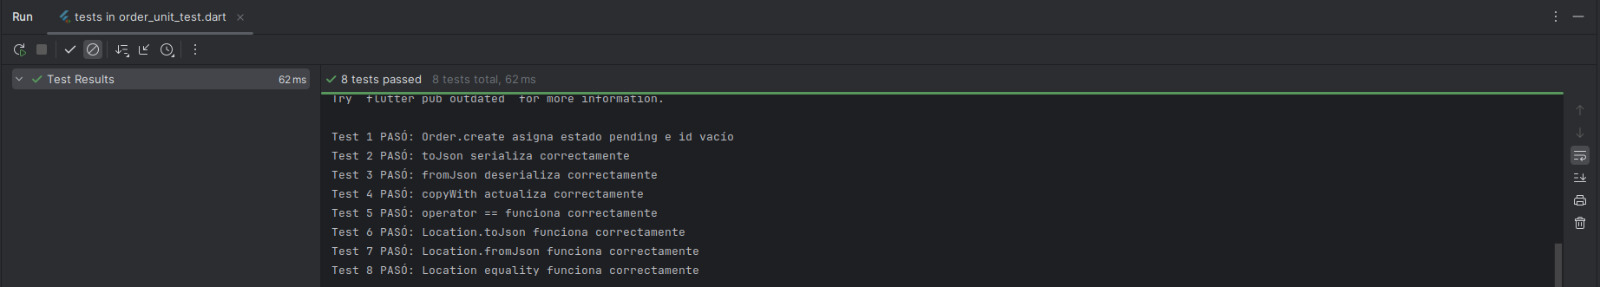
\includegraphics[width=0.8 \textwidth, height=10cm, keepaspectratio]{img/Test1.jpeg}
    \caption{Ejecución de pruebas unitarias}
    \label{fig:estructura1}
\end{figure}
